\documentclass[10pt, a4paper,final]{article}
\usepackage{graphicx}
%
%%%%%%%%%%%%%%%%%%%%%%%%%%%%%%%%%%%%%%%%%%%%%%%%%%%%%%%%%%%%%%%%%%%%%%%%%%%%
%   document style macros
%%%%%%%%%%%%%%%%%%%%%%%%%%%%%%%%%%%%%%%%%%%%%%%%%%%%%%%%%%%%%%%%%%%%%%%%%%%%
\def\Title#1{\begin{center} {\Large #1 } \end{center}}
\def\Author#1{\begin{center}{ \sc #1} \end{center}}
\def\Address#1{\begin{center}{ \it #1} \end{center}}
\def\andauth{\begin{center}{and} \end{center}}
\def\submit#1{\begin{center}Submitted to {\sl #1} \end{center}}
\newcommand\pubblock{\rightline{\begin{tabular}{l} Proceedings of DIS2022\\ 
         \pubdate  \end{tabular}}}

\newenvironment{Abstract}{\begin{quotation} \begin{center} 
             \large ABSTRACT \end{center}\bigskip 
      \begin{large}}{\end{large}\end{quotation}}

\newenvironment{Presented}{\begin{quotation} \begin{center} 
             PRESENTED AT\end{center}\bigskip 
      \begin{center}\begin{large}}{\end{large}\end{center} \end{quotation}}

\def\Acknowledgements{\bigskip  \bigskip \begin{center} \begin{large}
      \bf ACKNOWLEDGEMENTS \end{large}\end{center}}

%%%%%%%%%%%%%%%%%%%%%%%%%%%%%%%%%%%%%%%%%%%%%%%%%%%%%%%%%%%%%%%%%%%%%%%%%%%% 
%  personal abbreviations and macros
%    the following package contains macros used in this document:
%%%%%%%%%%%%%%%%%%%%%%%%%%%%%%%%%%%%%%%%%%%%%%%%%%%%%%%%%%%%%%%%%%%%%%%%%%%

\textwidth=6.5in
\textheight=8.75in
\hoffset=-0.85in
\voffset=-0.6in


% include packages you will need
\usepackage[utf8]{inputenc}
\usepackage{color}
\usepackage{lineno}
\usepackage{hyperref}
\usepackage[style=phys,%
	biblabel=brackets,%
	chaptertitle=false,pageranges=false,%
	maxnames=4,sorting=none]{biblatex}
\usepackage{amsmath,amsthm,amssymb}
\usepackage{graphicx}
\usepackage{physics}
\usepackage{subcaption}
\usepackage{tikz}
\usepackage{siunitx}
\usepackage{url}
\usepackage[obeyFinal]{todonotes}

\graphicspath{{images/}}
\addbibresource{references.bib}
%%%%%%%%%%%%%%%%%%%%%%%%%%%%%%%%%%%%%%%%%%%%%%%%%%%%%%%%%%%%%%%%%%%%
% basic data for the eprint:
%%%%%%%%%%%%%%%%%%%%%%%%%%%%%%%%%%%%%%%%%%%%%%%%%%%%%%%%%%%%%%%%%%%%


\newcommand\pubdate{\today}

%%  Affiliation
\def\affiliation{
On behalf of SeaQuest Collaboration, \\
Department of Physics, University of Illinois Urbana-Champaign, \\Urbana, Illinois 61801, USA}

%% Acknowledge the support
\def\support{\footnote{Work supported by NSF-2111046}}


\newcommand{\conference}{DIS2022: XXIX International Workshop on Deep-Inelastic Scattering and Related Subjects\\
Santiago de Compostela, Spain\\
May 2-6 2022}

\begin{document}
\large
\begin{titlepage}
	\pubblock


	\vfill
	\Title{Measurement of Charmonium Production in $p + p$ and $p + d$ Interaction in the Fermilab SeaQuest Experiment}
	\vfill

	\Author{Ching Him Leung \support}
	\Address{\affiliation}
	\vfill

	\begin{Abstract}
		SeaQuest has measured dimuon events from the interaction of \SI{120}{\GeV} proton
		beam on liquid hydrogen and deuterium targets with dimuon mass between \num{2}
		and \SI{8}{\GeV}. These dimuon events contain both the Drell-Yan process and the
		charmonium ($J/\psi$ and $\psi^\prime$) production. Unlike the Drell-Yan process
		which probes the antiquark distributions in the nucleons, the charmonium production
		is sensitive to both quark and gluon distributions. SeaQuest has extracted the
		$(p+d)/(p+p)$ cross section ratios as well as the differential cross sections for
		charmonium production in the kinematic region of $0.4 < x_F < 0.9$. The $(p+d)/(p+p)$
		cross section ratios for charmonium production are found to be significantly different
		from that of the Drell-Yan process. The measured differential cross sections for
		charmonium production are compared with theoretical model calculations.
	\end{Abstract}

	\vfill

	\begin{Presented}
		\conference
	\end{Presented}
	\vfill
\end{titlepage}

\setcounter{footnote}{0}
\normalsize


\section{Introduction}
\label{sec:intro}
The SeaQuest experiment at Fermilab was designed to measure high-mass dimuons
produced in the interaction of \SI{120}{\GeV} proton beam with various targets.
Dimuons originating from the Drell-Yan process \cite{drell1970} as well as the
decay of quarkonium states were collected simultaneously. Results from SeaQuest
on the $(p+d)/(p+p)$ Drell-Yan cross section ratios, which are sensitive to
the flavor asymmetry of $\bar{d}/\bar{u}$ in the proton, were reported recently
\cite{dove2021}.

\todo[inline]{$J/\psi$ production}
Unlike the Drell-Yan process which primarily involves the annihilation of quark
and antiquark pair via electromagnetic interaction, charmonium production proceeds
via strong interaction containing contributions from both quark-antiquark
annihilation and gluon-gluon fusion processes.

While proton-induced charmonium production is expected to be dominated by gluon-gluon
fusion process \cite{vogt1999}, some contributions form the quark-antiquark
annihilation process is also expected. The relative importance of these two
processes is expected to depends on the energy of the colliding hadron as well
as the Feynman-$x$ ($x_F$) of the charmonium \cite{peng1995}.


\section{E906/SeaQuest Experiment}
\label{sec:e906}
SeaQuest is a fixed-target experiment utilizing the \SI{120}{\GeV} proton beam
from the Fermilab Main Injector. Details of the SeaQuest spectrometer can be
found in Ref.~\cite{aidala2019}. The target system consists of seven
interchangeable targets, including a flask with liquid hydrogen, a flask with
liquid deuterium,an empty flask (vacuum), solid carbon, iron, and tungsten
targets as well as a space with no target (air). The targets are interchanged
periodically to reduce systematic uncertainties in the measured cross section
ratios for different targets.

The spectrometer consists of two magnets and four tracking stations. FMag,
placed \SI{104}{\cm} downstream the target, is a \SI{5}{\m} solid iron magnet
that acts as the beam dump as well as a focusing magnet. It is then followed by
the first tracking stations. Stations 1, 2 and 3 each consists of plastic
scintillator hodoscopes and drift chambers. An open air dipole magnet (KMag) is
placed between station 1 and station 2. The vertical magnetic field from both
magnets bends the muons horizontally, allowing the measurement of the momentum
of the muons. Downstream of station 3, there is a 1 m iron wall acting as a
hadron absorber. Station 4 is located behind the hadron absorber and acts as a
muon identifier. Station 4 consists of a hodoscope array and 4 layers of
proportional tube planes. Tracks that pass through the hadron absorber and
produce hits on station 4 are assumed to be from muons.

\section{Extraction of \texorpdfstring{$J/\psi$}{J/psi} cross section}
\label{sec:result}
Data collection for SeaQuest ran from April 2014 to July 2017. The analysis
presented here is performed on data collected until August 2015, about half
of the entire data set. After applying various analysis cuts to select
candidate dimuon events form the liquid hydrogen target, the dimuon invariant
mass distribution is shown in Fig.~\ref{fig:mass}. The mass distribution is
fitted by taking into account several contributions. First, the mass spectrum
from the data collected with the empty target flask, properly normalized by
the integrated beam intensity. Second the expected mass distributions for
$J/\psi$ and $\psi^\prime$ are  obtained by studying the GEANT4 based Monte-Carlo
simulation, which takes into account the spectrometer acceptance. The Drell-Yan
line shape is also generated using a similar procedure with the thrown distribution
generated using a next-to-leading order calculation and CT14 parton distributions.
The random background is then simulated by using the data collected with a
``single-muon '' trigger. The two ``single-muon'' events are combined to
create a simulated ``dimuon'' events, which is then sent through the same
analysis chain. The data is then fitted to a sum of these different
components to obtained the relative normalization for each components. The
data are well described by this fitting procedure. And the mass distribution
in each kinematic bin is also well described by this fitting procedure.

\begin{figure}[htbp!]
	\centering
	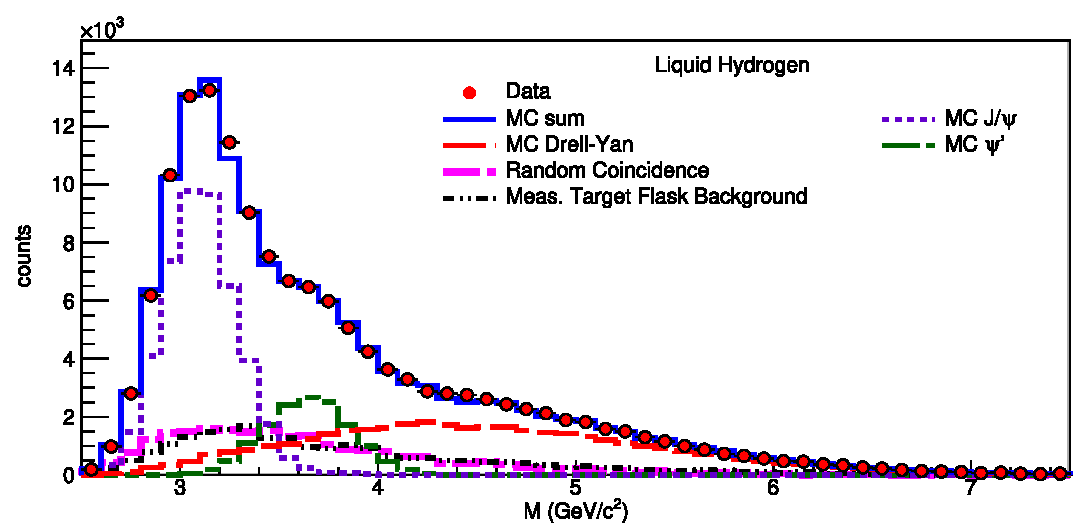
\includegraphics[width=0.65\linewidth]{extFig3_LH2}
	\caption{The reconstructed invariant mass distribution for data collected on
		liquid hydrogen target after all analysis cuts \cite{dove2021}.
		In the lower mass region, the predominant signal is produced by the decay
		of $J/\psi$ and $\psi^\prime$. }
	\label{fig:mass}
\end{figure}

After the number of $J/\psi$ events is extracted from the mass distributions,
the quarkonium production cross section is obtained from the yeilds as follows
\begin{equation}
	B\dv{\sigma}{c_F} = \frac{N_{\textrm{events}}}{\Delta x_F \mathcal{L} \epsilon},
\end{equation}
where $B$ is the branching ratio for $J/\psi$ to decay into a muon pair,
$epslon$ is the spectrometer acceptance and efficiency correction, and
$\mathcal{L}$ is the effective luminosity. The spectrometer acceptance and
efficiency correction are obtained by studying the Monte-Carlo simulation.

To compare the measured $J/\psi$ production cross section with theoretical
expectations, we have performed calculation using the Next-to-Leading
order (NLO) Color Evaporation Model (CEM)\cite{mangano1993} and
Non-Relativistic QCD (NRQCD) \cite{bodwin1997}. In both model, the heavy
quark-antiquark ($\bar{Q}Q$) pair production via various QCD hard process
is calculated using purturbative QCD. The main difference between the two
models is in the hadronization into specific quarkonium bound state.
In the CEM framework, $\bar{c}c$ pair with an invariant mass $M_{\bar{c}c}$
smaller than the $D\bar{D}$ open-charm threshold, a constant probability $F$,
specific for each charmonium state, accounts for the hadronization into
colorless charmonium state. In contrast, in NRQCD, the hadronization is
described by a set of long-distance matrix elements which depend on the spin,
color and angular momentum of the $\bar{Q}Q$ pairs.

The model predictions from both model for the $J/\psi$ production with a \SI{120}{\GeV}
proton beam are shown in Fig.~\ref{fig:jpsi_theory}. At forward $x_F$, both models suggest
that quark-antiquark annihilation being more important than gluon-gluon fusion, but NRQCD
put greater importance on quark-antiquark annihilation.
\begin{figure}[htbp!]
	\centering
	\begin{subfigure}{0.45\linewidth}
		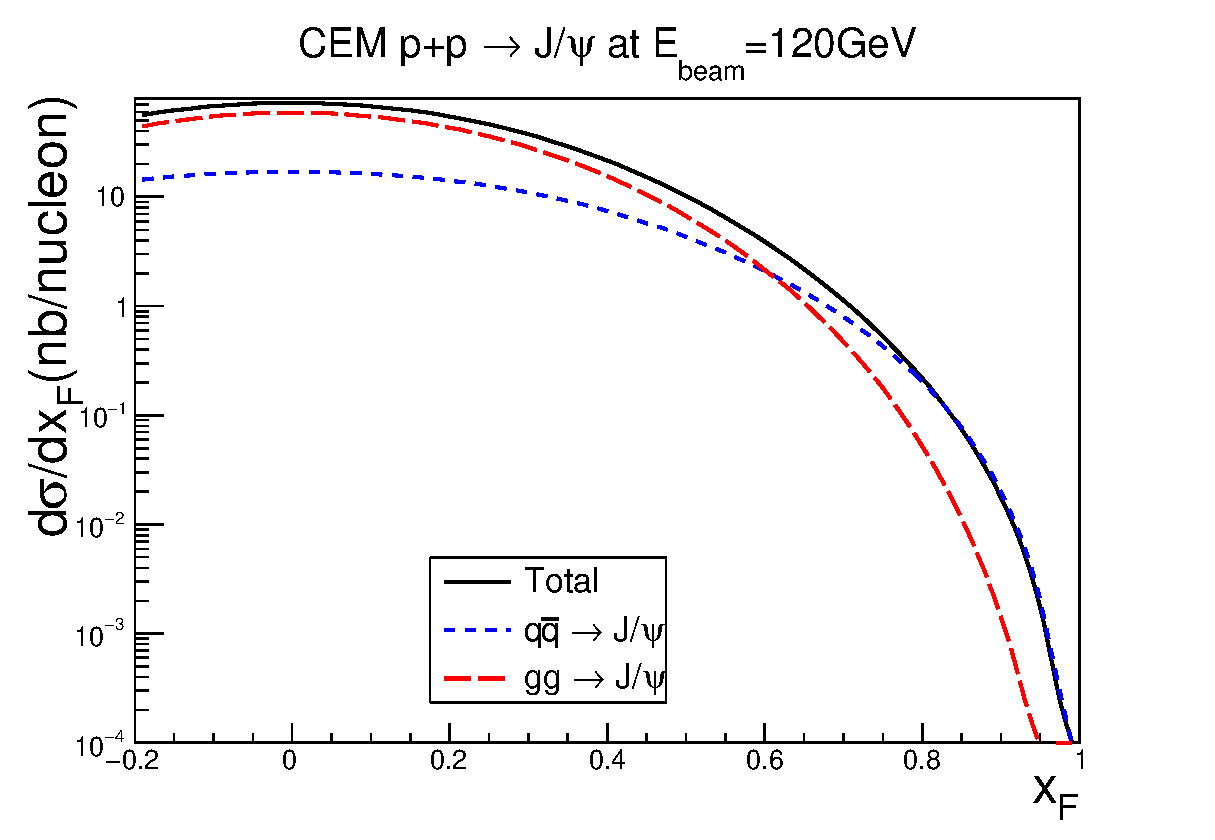
\includegraphics[width=0.9\linewidth]{pp_norm_cs_NLO_pp}
	\end{subfigure}
	\begin{subfigure}{0.45\linewidth}
		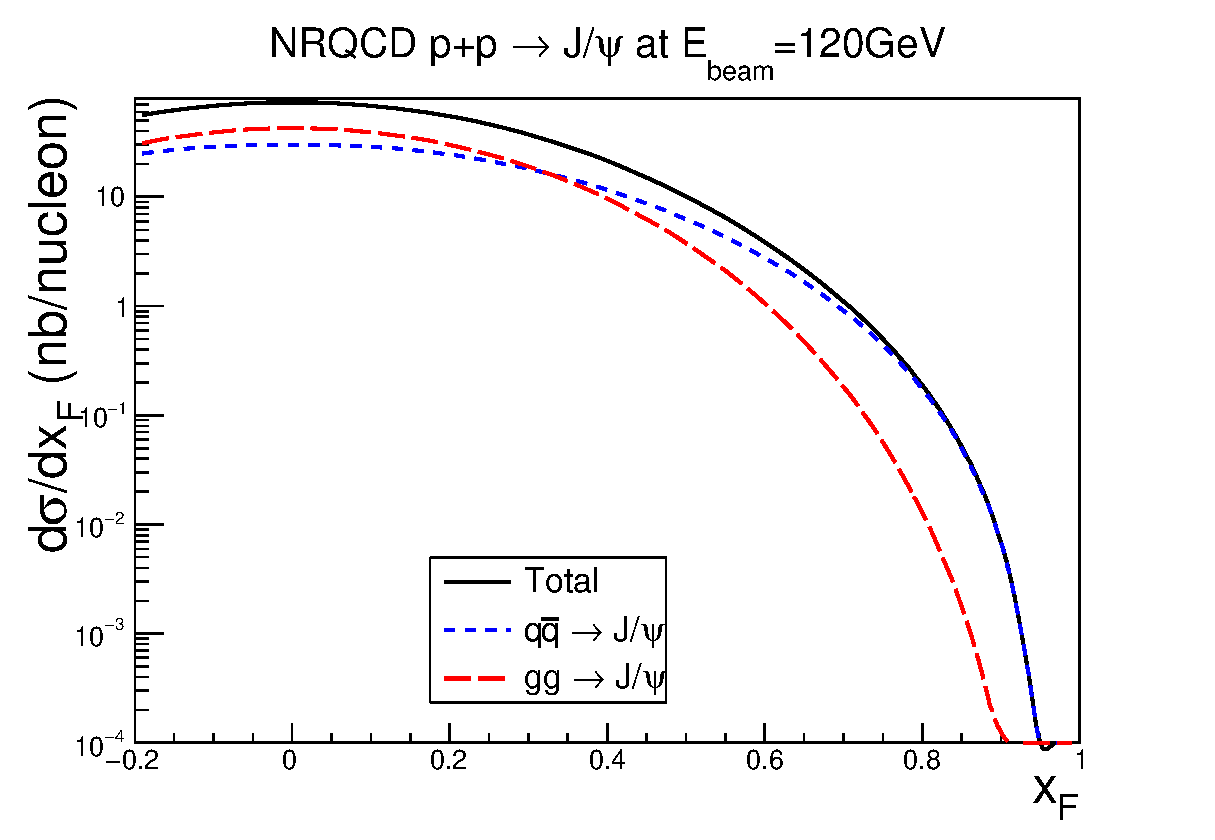
\includegraphics[width=0.9\linewidth]{jpsi_cs_pp}
	\end{subfigure}
	\caption{The model prediction for $J/\psi$ production with a \SI{120}{\GeV}
		proton beam using CEM (left) and NRQCD {right}. Contribution from the
		quark-antiquark annihilation and gluon-gluon fusion are shown as blue dotted line
		and red dashed line.}
	\label{fig:jpsi_theory}
\end{figure}

The preliminary result from SeaQuest is shown in Fig.\ref{fig:abs_cs_NRQCD},
and are compared with both the CEM and NRQCD calculation. The main sources
of systematic uncertainties comes from the modeling of the random background
and the beam luminosity normalization. The normalization of the CEM calculation is
adjusted to fit the data, and account for the hadronization probability. The line
shape of the extracted cross section is in good agreement with CEM. For the NRQCD
calculation, the LDMes are taken from \cite{hsieh2021}, which are extracted from
a global analysis of pion and proton induced charmonium production in fixed target
experiments. The overall normalization and the line shape of the extracted cross
section are also in good agreement with the NRQCD calculation.
\todo{describe the cross section calculation and systematic}
\begin{figure}[htbp!]
	\centering
	\begin{subfigure}{0.45\linewidth}
		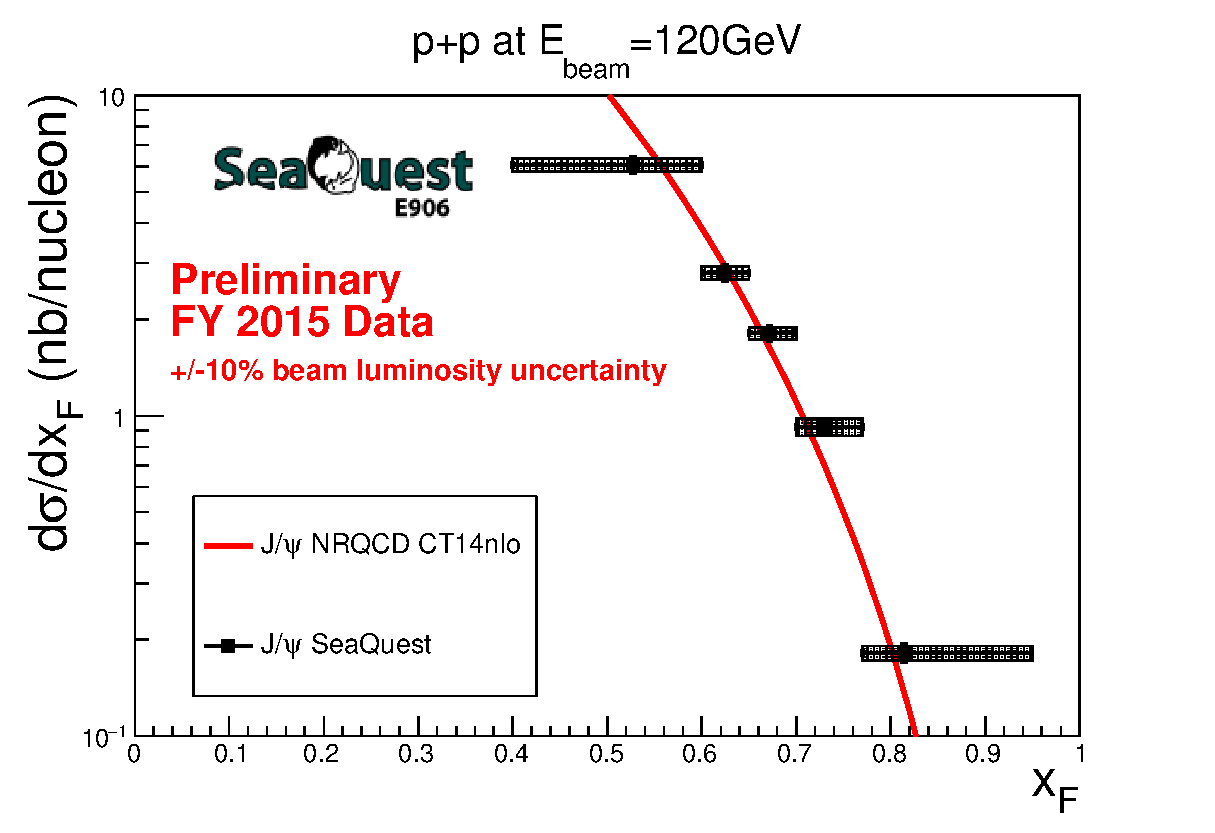
\includegraphics[width=0.9\linewidth]{jpsi_xF_LH2}
	\end{subfigure}
	\begin{subfigure}{0.45\linewidth}
		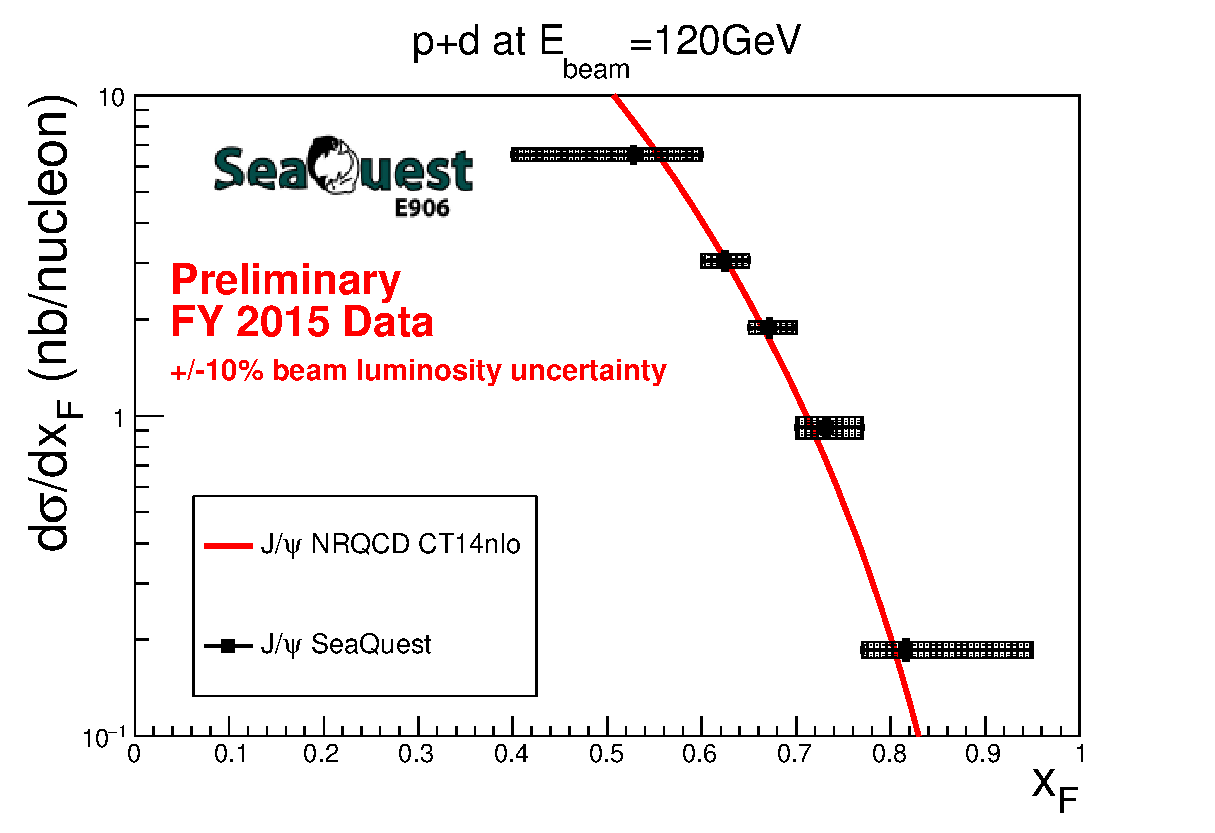
\includegraphics[width=0.9\linewidth]{jpsi_xF_LD2}
	\end{subfigure}\\
	\begin{subfigure}{0.45\linewidth}
		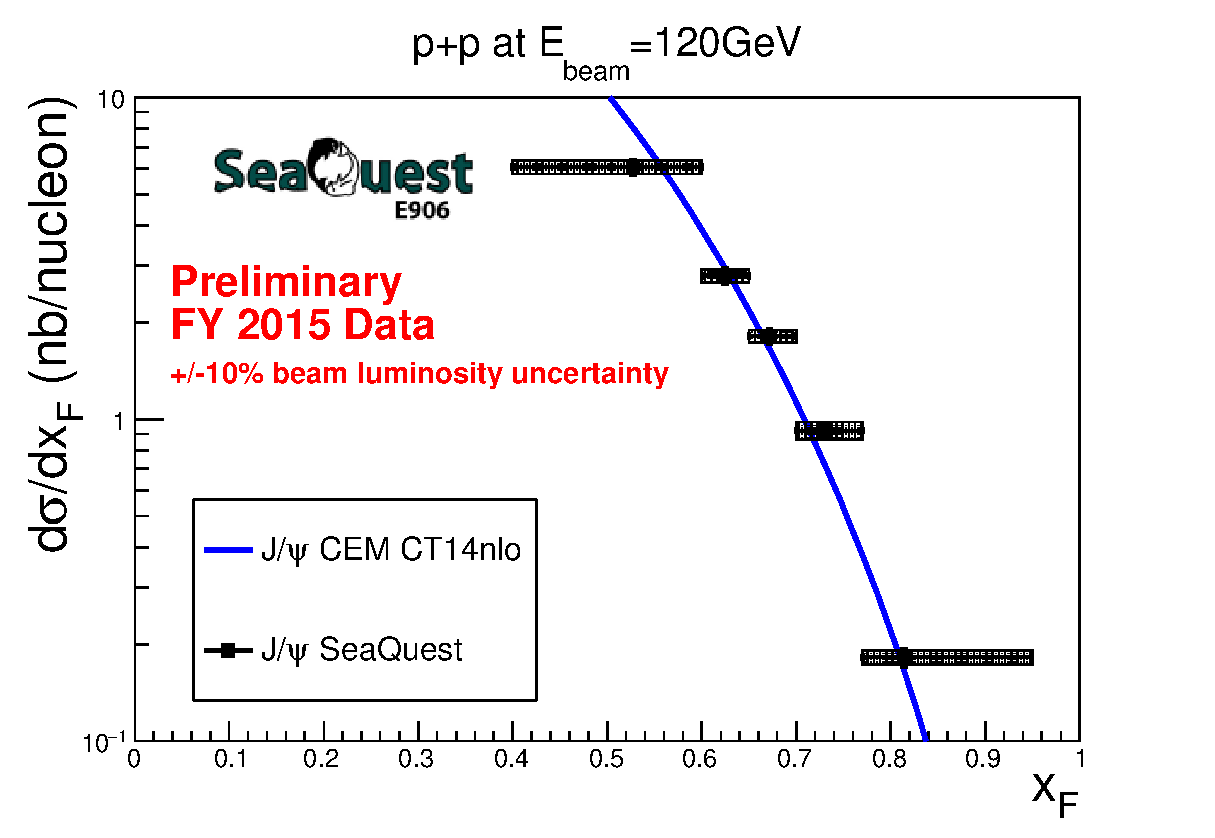
\includegraphics[width=0.9\linewidth]{jpsi_xF_LH2_CEM}
	\end{subfigure}
	\begin{subfigure}{0.45\linewidth}
		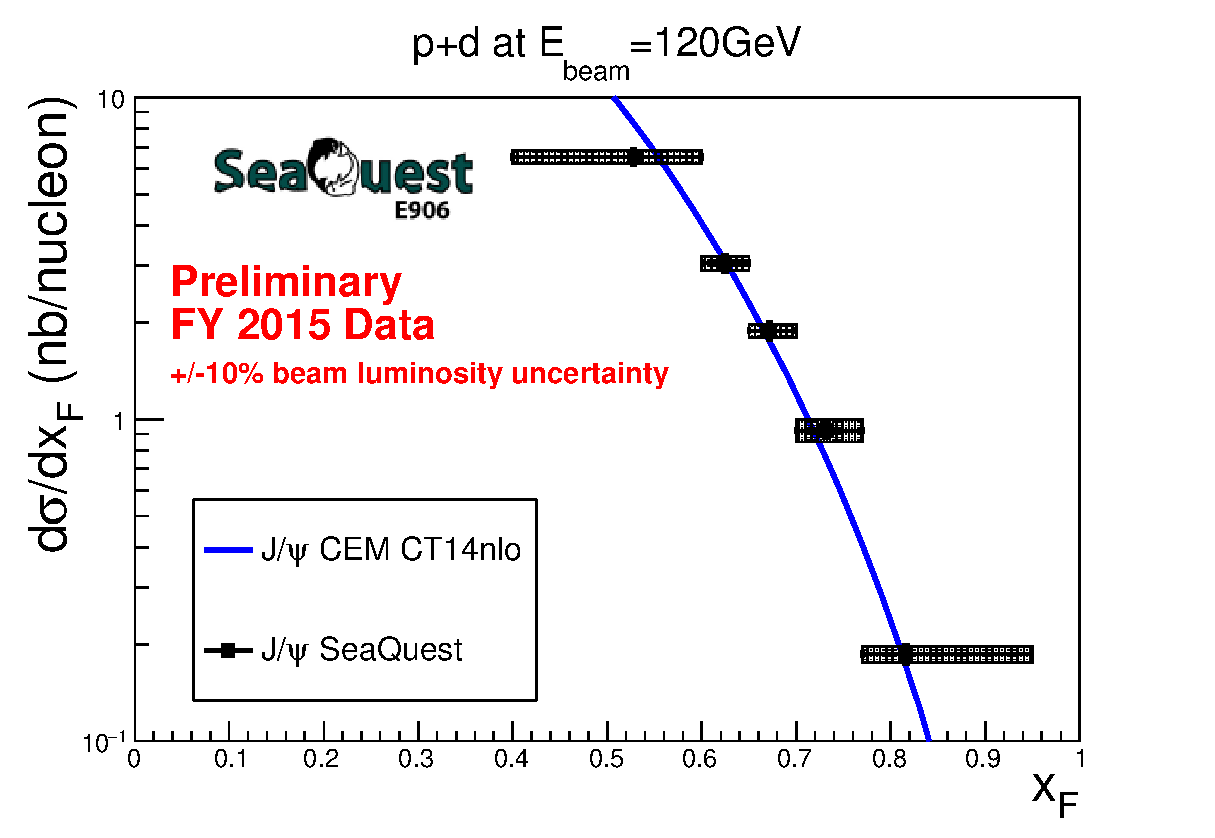
\includegraphics[width=0.9\linewidth]{jpsi_xF_LD2_CEM}
	\end{subfigure}
	\caption{The preliminary result on the extracted $J/\psi$ cross section for
		proton on hydrogen (left) and proton on deuterium (right). The result is
		also compared with NRQCD predictions (top) and CEM prediction (bottom).}
	\label{fig:abs_cs_NRQCD}
\end{figure}


The $(p+d)/2(p+p)$ cross section ratio can also be obtained. As the most of the
systematic uncertainties are correlated between the hydrogen and deuterium targets,
they would cancel out in the ratios.
\begin{figure}[htbp!]
	\centering
	\begin{subfigure}{0.45\linewidth}
		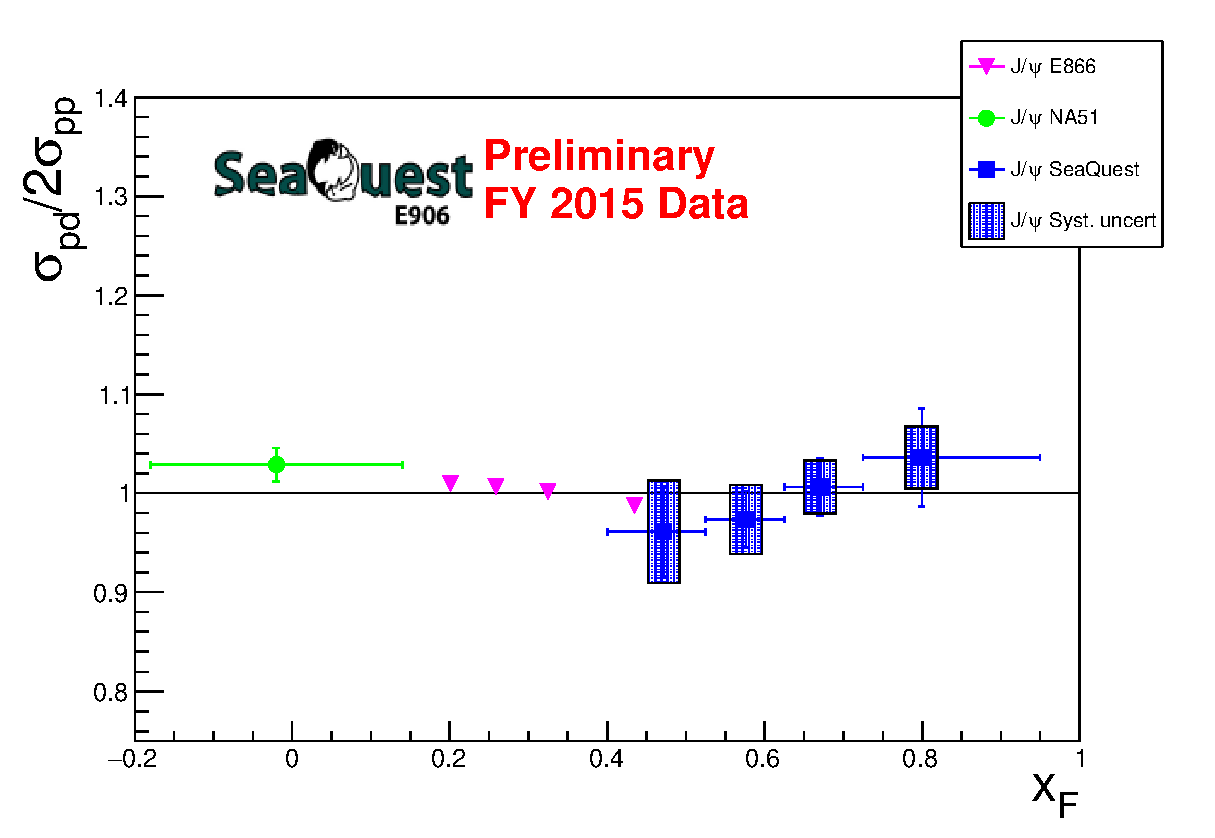
\includegraphics[width=0.9\linewidth]{jPsi_all_noTheory_v2}
	\end{subfigure}
	\begin{subfigure}{0.45\linewidth}
		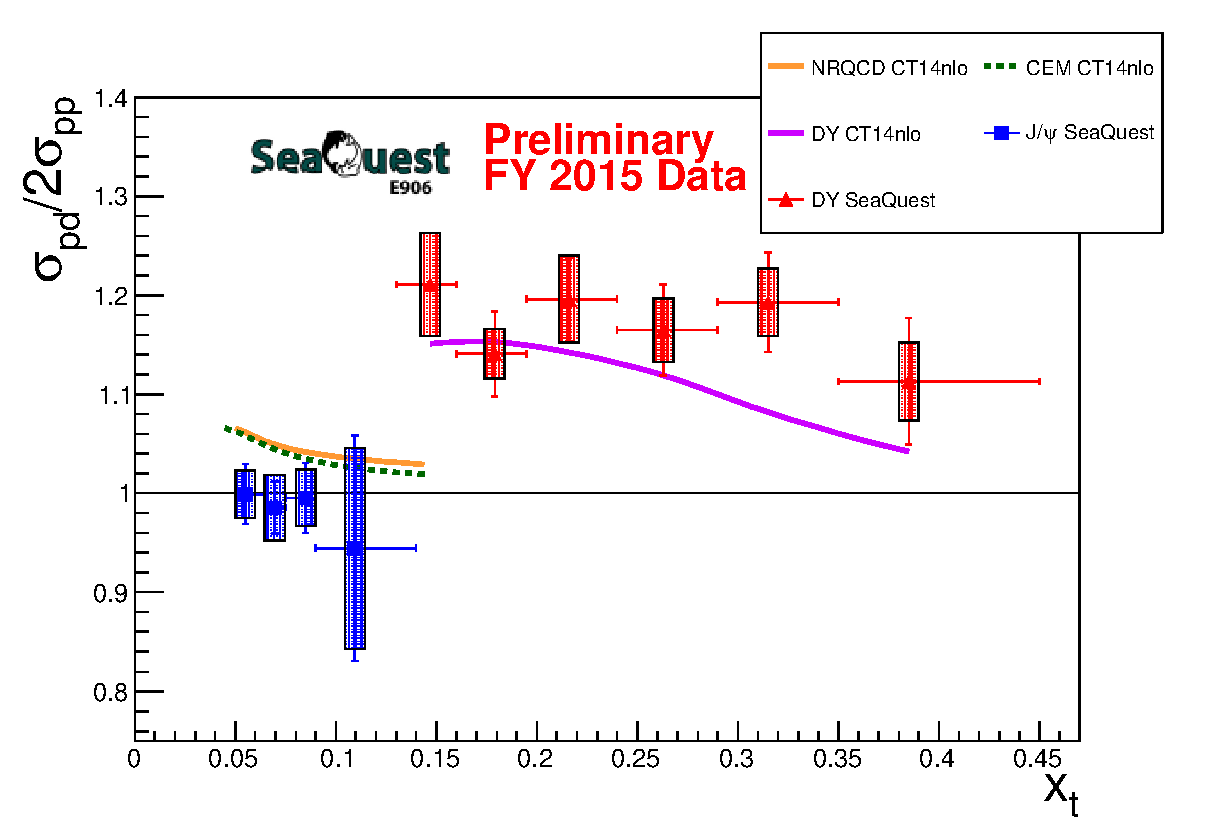
\includegraphics[width=0.9\linewidth]{jPsi_csr_x2_nature_NRQCD_CEM}
	\end{subfigure}
	\caption{The preliminary result on the extracted $J/\psi$ $(p+d)/2(p+p)$
		cross section ratio as a function of $x_F$ (left) and $x_t$ (right).
		The extracted ratio is also compared with previous measurements by NA51
		\cite{abreu1998} and E866 \cite{peng2003} (left), as well as the Drell-Yan
		cross section ration reported by SeaQuest\cite{dove2021} (right).}
	\label{fig:csr}
\end{figure}
The preliminary $J/\psi$ $(p+d)/2(p+p)$ cross section ratio is shown in
Fig.~\ref{fig:csr}. The SeaQuest measurement is at a lower energy and higher $x_F$
compared to previous measurements. The preliminary result is consistent with unity
within uncertainty, in qualitative agreement with earlier measurement at \SI{450}{\GeV}
by the NA51 Collaboration and \SI{800}{\GeV} by the E866 Collboration.

While the Drell-Yan process proceeds via electromagnetic interaction sensitive
to the quarks and antiquarks distribution, the charmonium production is a strong
interaction sensitive to the gluon contents of the colliding nucleons. These
different characteristics between the two processes are reflected in the
$(p+d)/2(p+p)$ ratios. While Drell-Yan ratios is significantly different from unity
as a result of the flavor asymmetry of the light-quark sea, the $J/\psi$ production
cross section ratio is consistent with unity.

The CEM and NRQCD calculation are shown as green dotted line and orange solid line
respectively. The difference between the two calculations are reflecting the higher
importance of the quark-antiquark annihilation in the NRQCD calculation.

\section{Conclusions}
The simultaneous measurement of the charmonium production and the Drell-Yan dimuons
in the SeaQuest experiment allows for a comparison of the two distict process. The
extracted $J/\psi$ production cross section is in good agreement with both the CEM
and NRQCD calculation. The $(p+d)/2(p+p)$ $J/\psi$ production cross section ratio
is consistent with unity, and the difference between the $J/\psi$ and Drell-Yan
ratio is reflecting the different mechanism between the two process.

Predictions from the NRQCD calculation suggest the quark-antiquark annihilation would
be more important in the $\psi^\prime$ production, and hence one would expect $\psi^\prime$
to have a boarder $x_F$ distribution to $J/\psi$. The extraction of the $\psi^\prime$
cross section is currently underway and would be able to provide input to charmonium
production. Furthermore, the data from the remaining data sets would roughly double
the statistics for both the charmonium production as well as the Drell-Yan.

\printbibliography[heading=bibintoc,title={References}]
\listoftodos
\end{document}

